\section{Landing Page Implementation}
The landing page serves as the primary entry point for the platform, separated into distinct, self-contained functional React components integrated within the main layout container.

\subsection{HomePage Layout and Global Styling}

\textbf{Purpose:} Acts as the root orchestrator for the landing page, aggregating all functional sections sequentially and injecting the global design tokens.

\vspace{0.2cm}
\noindent\textbf{Location:} \texttt{src/pages/Home/HomePage.jsx}

\vspace{0.2cm}
\noindent\textbf{Notes:}
\begin{itemize}
    \item Serves as the primary parent container, importing and rendering \texttt{HomeNavbar}, \texttt{HomeHero}, \texttt{HomeAbout}, \texttt{HomeServices}, \texttt{HowItWorks}, \texttt{HomeMeetUs}, and \texttt{HomeFooter}.
    \item Injects global stylesheets (\texttt{variables.css} and \texttt{base.css}) at the root level to enforce a consistent design language application-wide.
    \item Relies on CSS variables (e.g., \texttt{--body-background}, \texttt{--text-color}) controlled by a global \texttt{[data-theme="dark"]} selector, ensuring seamless transitions between light and dark modes.
    \item Standardizes shared UI elements—such as primary gradient buttons (\texttt{.btn-primary-floo}), section eyebrow tags (\texttt{.section-tag}), and \texttt{Audiowide} typography—to prevent code duplication across child components.
\end{itemize}

\subsection{Shared Content Configuration}

\textbf{Purpose:} Centralizes all textual content and static data arrays used across the landing page to ensure maintainability and strict separation of presentation logic from copy.

\vspace{0.2cm}
\noindent\textbf{Location:} \texttt{src/pages/Home/homeConstants.js}

\vspace{0.2cm}
\noindent\textbf{Notes:}
\begin{itemize}
    \item Consolidates copy for the Hero, About, Services, Video, and Meet Us sections into a single exported \texttt{HOME\_TEXT} object.
    \item Allows developers to easily update platform messaging, titles, and descriptions without needing to parse or modify complex JSX structures.
    \item Maps dynamic keys (such as service icon identifiers) within data arrays, keeping the rendering files clean and focused solely on UI logic.
\end{itemize}

\subsection{HomeNavbar Component}

\textbf{Purpose:} Provides site-wide navigation, handles user authentication state rendering, and toggles the global light/dark theme.

\vspace{0.2cm}
\noindent\textbf{Location:} \texttt{src/pages/Home/components/HomeNavbar.jsx}

\vspace{0.2cm}
\noindent\textbf{Notes:}
\begin{itemize}
    \item Integrates with the global \texttt{UserContext} to conditionally render Sign In/Up options for guests, or a profile avatar for authenticated users.
    \item Utilizes a custom \texttt{ModeSwitch} to toggle root CSS variables, ensuring seamless transition between light and dark visual states.
    \item Implements a sticky, glassmorphic layout that responds dynamically to the vertical scroll state.
\end{itemize}

\subsection{HomeHero Component}

\textbf{Purpose:} Establishes the initial user context using typography reveals and physics-driven, interactive background elements.

\vspace{0.2cm}
\noindent\textbf{Location:} \texttt{src/pages/Home/components/HomeHero.jsx}

\vspace{0.2cm}
\noindent\textbf{Notes:}
\begin{itemize}
    \item A dynamic background graphic tracks cursor movement using Framer Motion's \texttt{useMotionValue} and \texttt{useSpring} hooks.
    \item Applies a spring dampening effect to smooth pointer input into fluid coordinate translations on the screen.
\end{itemize}

\begin{figure}[h!]
    \centering
    
\includegraphics[width=0.95\textwidth]{images/home-page/home-hero-image.png}
\end{figure}

\subsection{HomeAbout Component}

\textbf{Purpose:} Introduces the platform's value proposition utilizing a responsive two-column grid and dynamic, scroll-driven parallax effects.

\vspace{0.2cm}
\noindent\textbf{Location:} \texttt{src/pages/Home/components/HomeAbout.jsx}

\vspace{0.2cm}
\noindent\textbf{Notes:}
\begin{itemize}
    \item Implements a depth-enhancing parallax effect natively using Framer Motion's \texttt{useScroll} and \texttt{useTransform} hooks, mapping viewport scroll progress directly to the Y-axis position, scale, and rotation of the visual asset.
    \item Features staggered, viewport-triggered entrance animations (\texttt{whileInView}) utilizing custom animation variants (\texttt{fadeUp}) for smooth typography reveals.
    \item Structured using a custom CSS Grid layout (\texttt{1fr 1fr}) that collapses gracefully to a single column on mobile viewports.
    \item Explicitly avoids \texttt{overflow: hidden} on the parent container to ensure the scroll-linked parallax travel and the bottom pulsating chip indicator are not clipped.
\end{itemize}


\begin{figure}[h!]
    \centering
    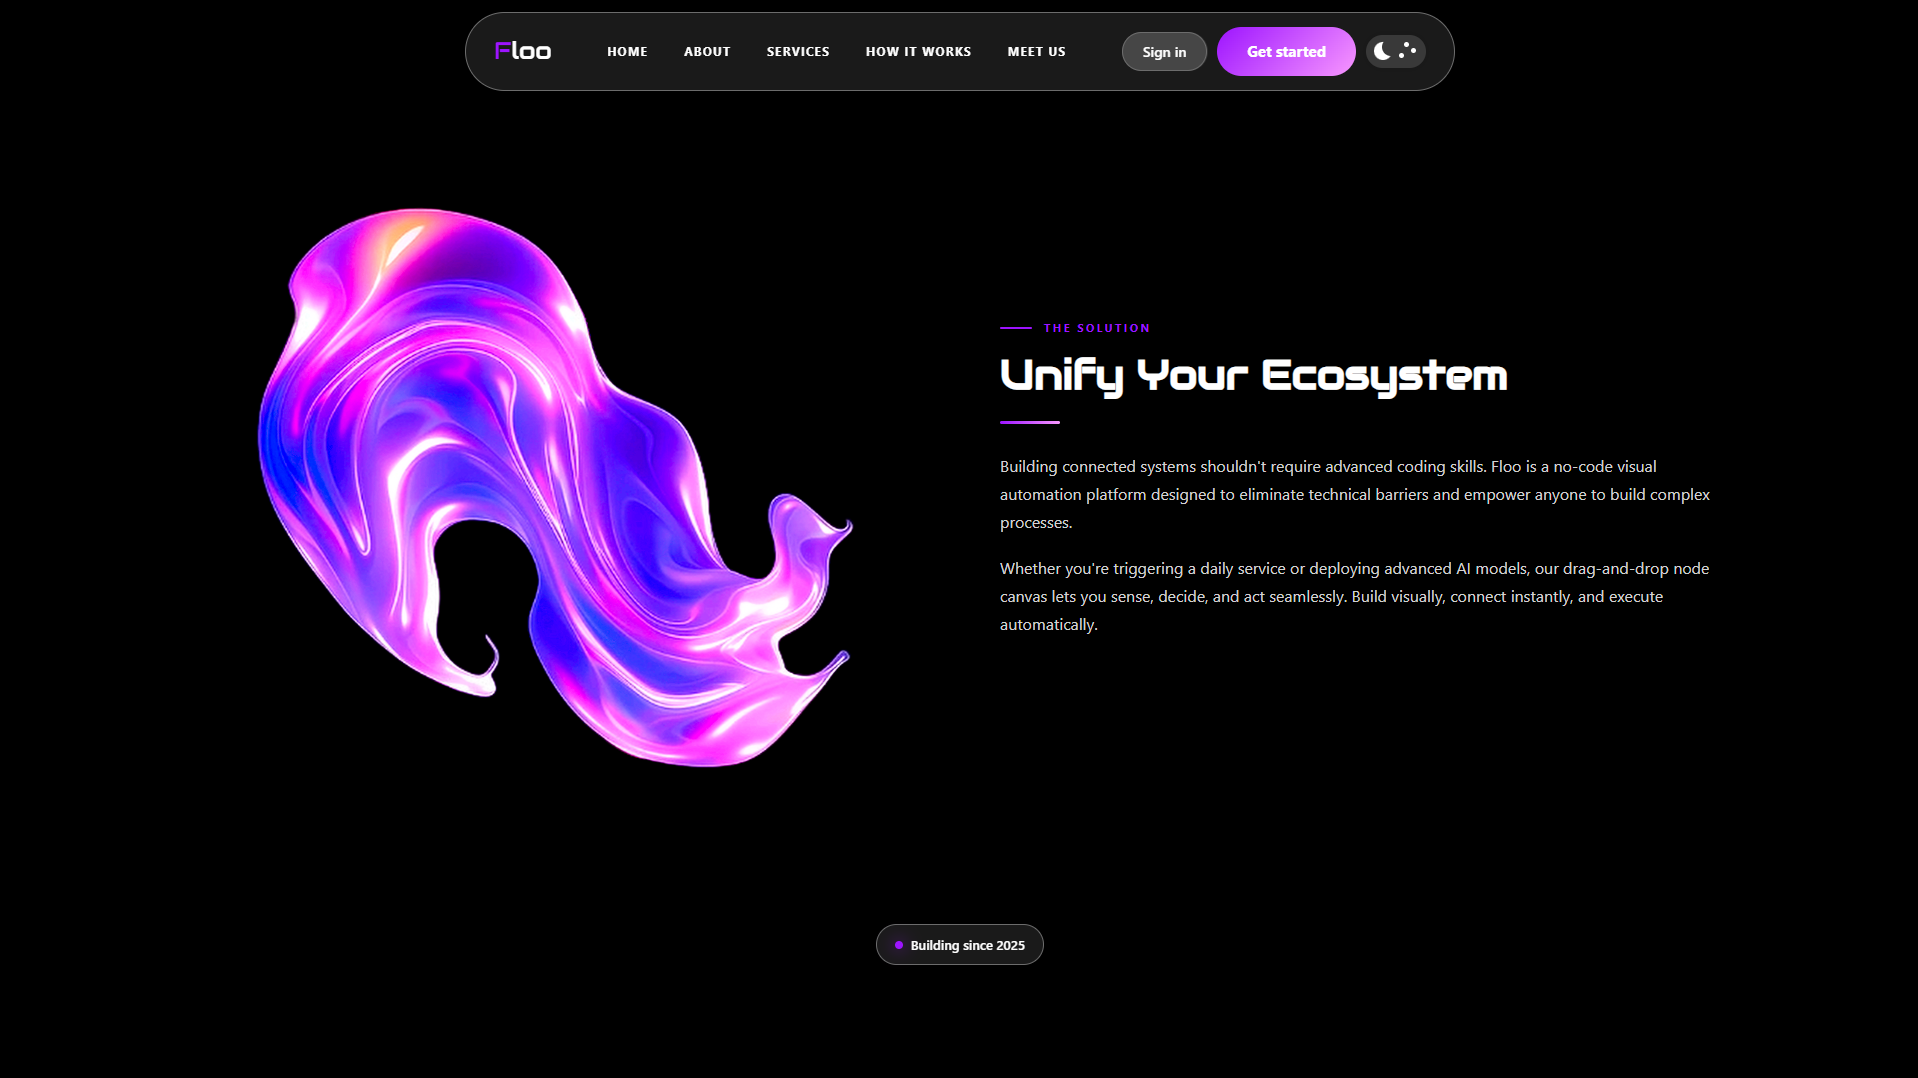
\includegraphics[width=0.95\textwidth]{images/home-page/home-about-image.png}
\end{figure}

\subsection{HomeServices Component}

\textbf{Purpose:} Presents the platform's core features via interactive, kinematic 3D tilt cards.

\vspace{0.2cm}
\noindent\textbf{Location:} \texttt{src/pages/Home/components/HomeServices.jsx}

\vspace{0.2cm}
\noindent\textbf{Notes:}
\begin{itemize}
    \item Maps the cursor's continuous 2D screen coordinates directly to rotational deformation angles on the card element.
    \item Produces a tactile 3D rotation paired with a dynamic, mouse-following radial CSS background gradient acting as a virtual spotlight.
\end{itemize}

\begin{figure}[h!]
    \centering
    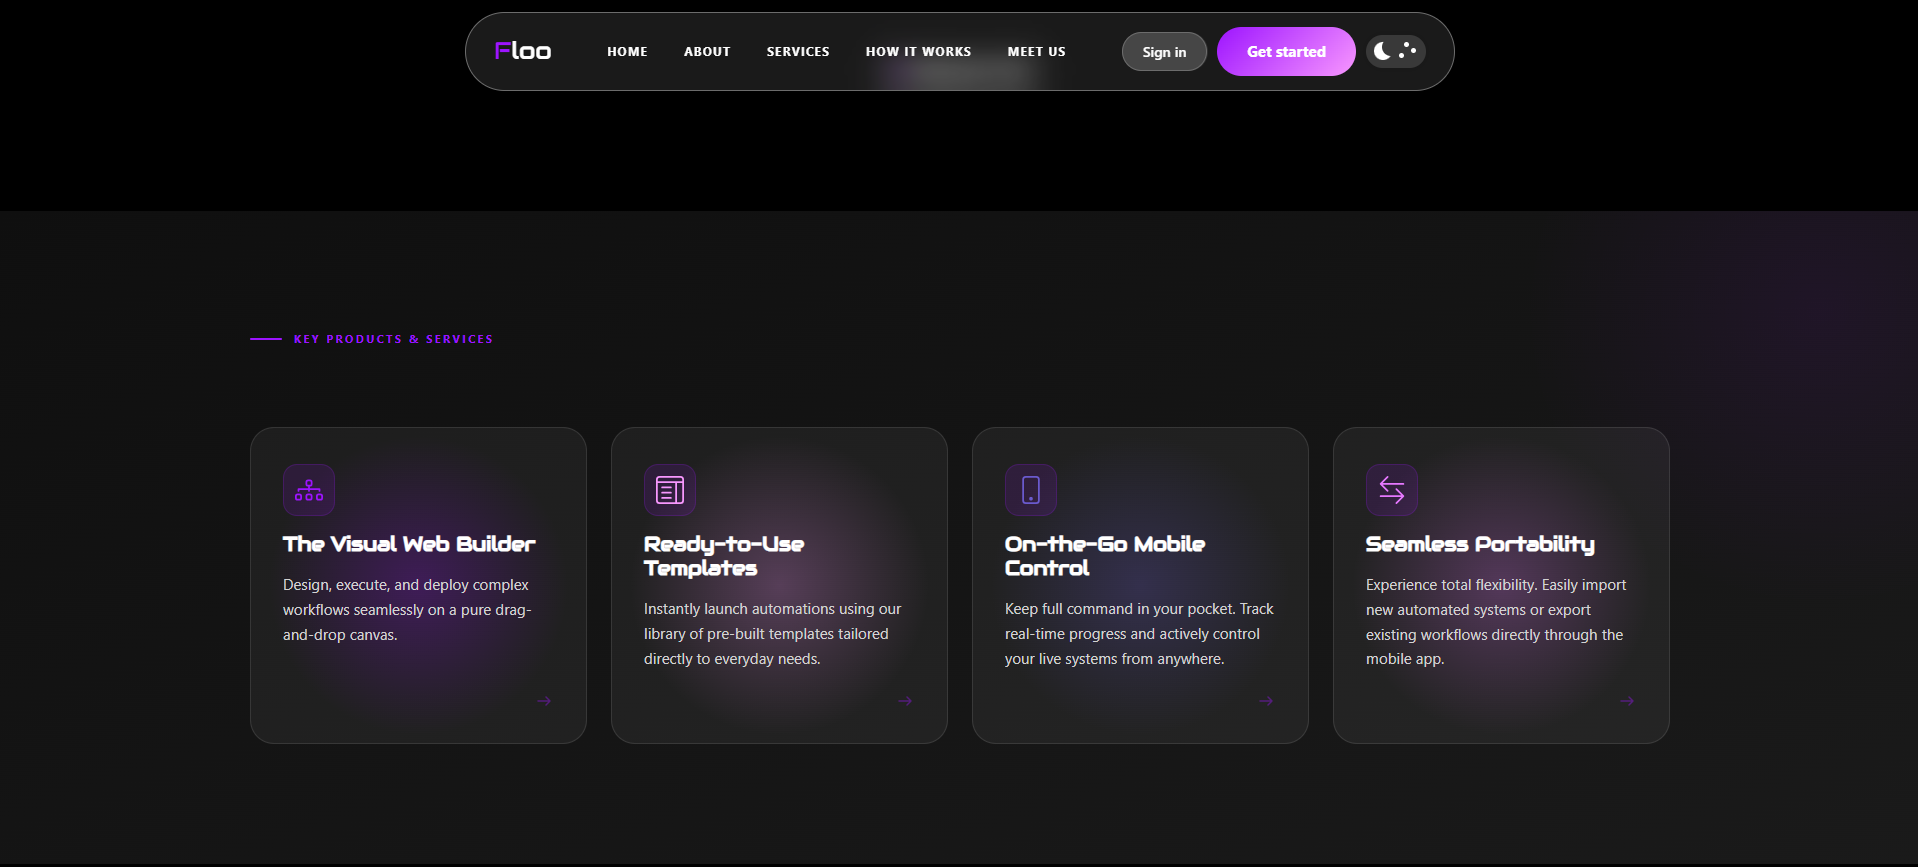
\includegraphics[width=0.95\textwidth]{images/home-page/home-services-image.png}
\end{figure}

\subsection{HowItWorks Component}

\textbf{Purpose:} Displays a product demonstration video with custom-built, interactive playback controls and scroll-triggered entrance animations.

\vspace{0.2cm}
\noindent\textbf{Location:} \texttt{src/pages/Home/components/HowItWorks.jsx}

\vspace{0.2cm}
\noindent\textbf{Notes:}
\begin{itemize}
    \item Utilizes React's \texttt{useRef} hook to securely target and manipulate the HTML5 \texttt{<video>} element for native play and pause functionality.
    \item Implements dynamic state tracking (\texttt{isPlaying} and \texttt{hasPlayed}) to transition a custom play button from the dead-center of the video to the bottom-right corner after the user's initial interaction.
    \item Wraps the video container and headers in Framer Motion components to trigger smooth fade-ins and vertical translations exactly when the section enters the user's viewport.
    \item Uses a visually appealing radial gradient backdrop (\texttt{.video-glow-backdrop}) combined with CSS blurs to create a glowing lighting effect behind the video wrapper.
\end{itemize}

\begin{figure}[h!]
    \centering
    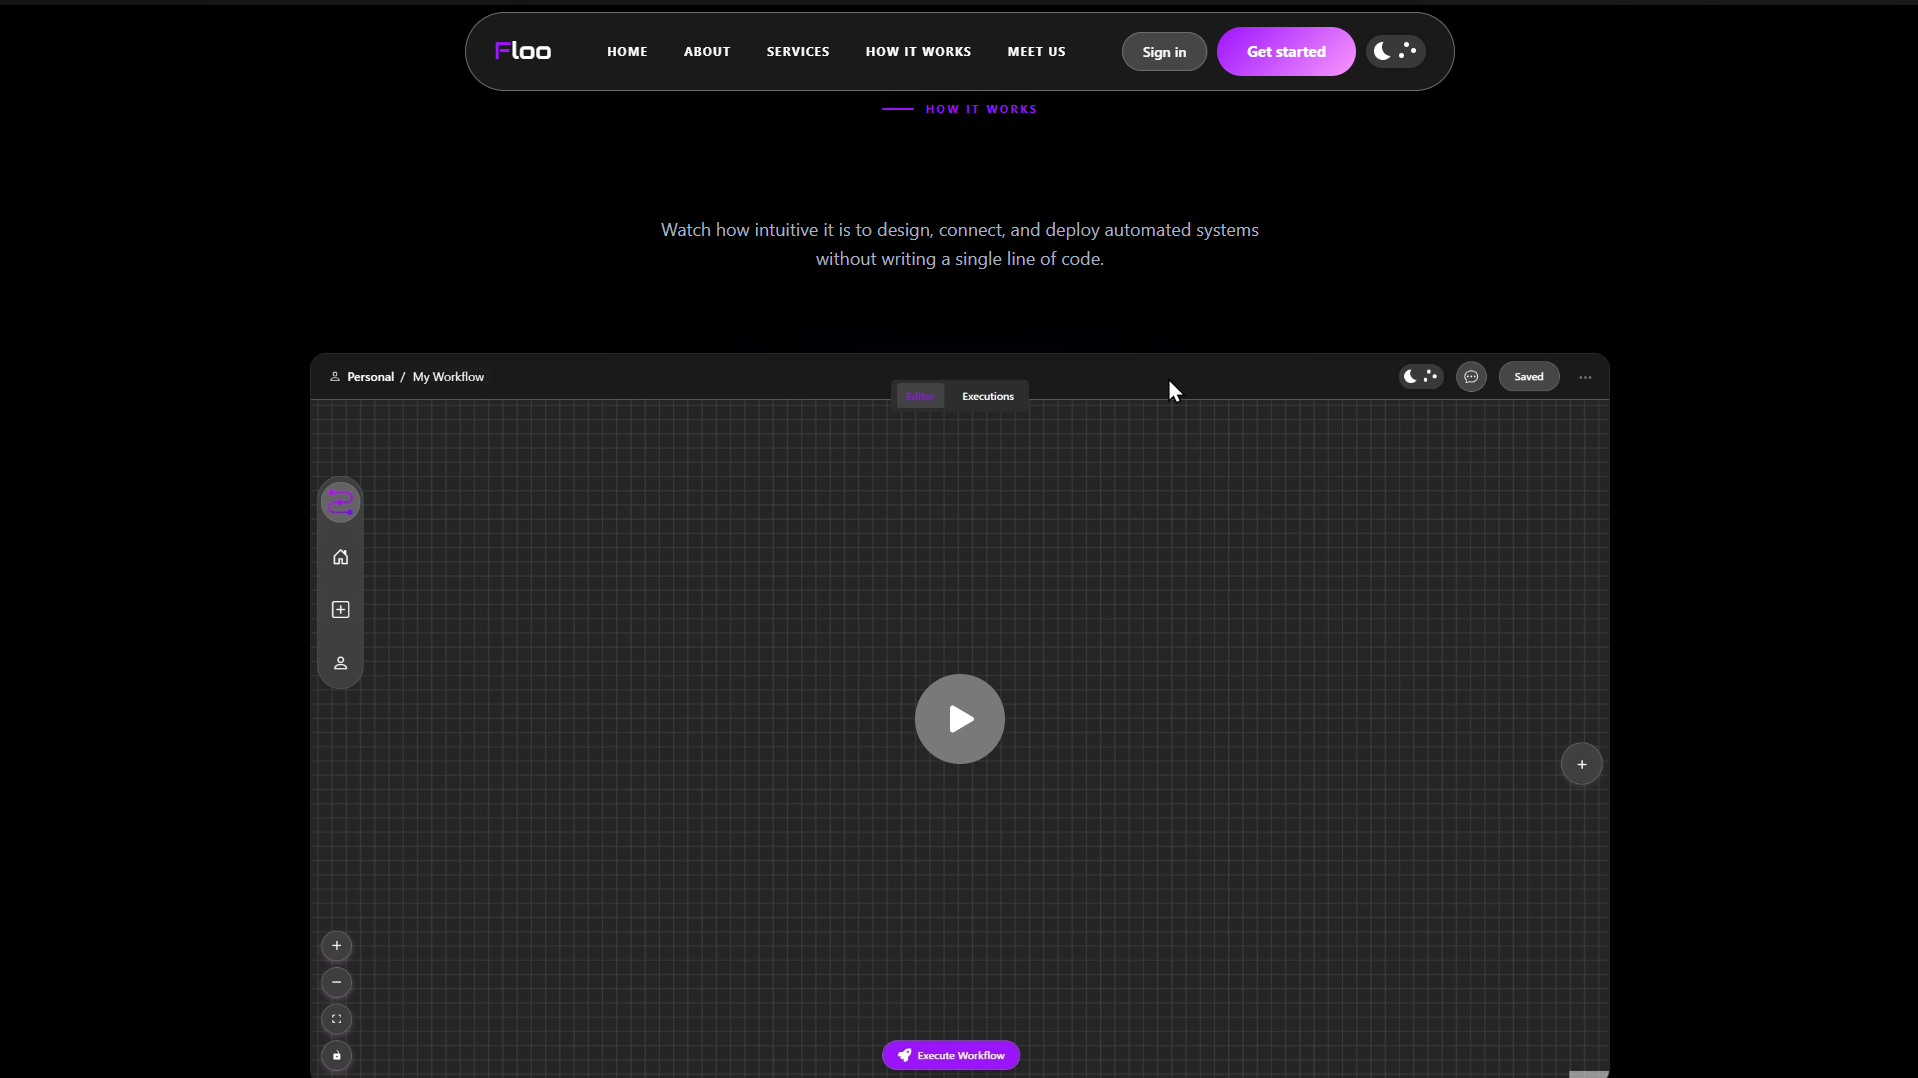
\includegraphics[width=0.95\textwidth]{images/home-page/home-howitworks-image.png}
\end{figure}

\subsection{HomeMeetUs Component}

\textbf{Purpose:} Displays a responsive, infinite-looping carousel to showcase the development team members.

\vspace{0.2cm}
\noindent\textbf{Location:} \texttt{src/pages/Home/components/HomeMeetUs.jsx}

\vspace{0.2cm}
\noindent\textbf{Notes:}
\begin{itemize}
    \item Utilizes the Swiper library for core carousel functionality.
    \item Relies on hardware-accelerated CSS transitions and glassmorphic filtering.
    \item The layout scales dynamically, shifting from a single column on mobile devices up to three simultaneous slides on larger viewports.
\end{itemize}

\begin{figure}[h!]
    \centering
    
\includegraphics[width=0.95\textwidth]{images/home-page/home-meetus-image.png}
\end{figure}

\subsection{HomeFooter Component}

\textbf{Purpose:} Encapsulates site navigation links and features a continuous, linear typography marquee.

\vspace{0.2cm}
\noindent\textbf{Location:} \texttt{src/pages/Home/components/HomeFooter.jsx}

\vspace{0.2cm}
\noindent\textbf{Notes:}
\begin{itemize}
    \item Controlled by uniform linear velocity transformations along the X-axis for a seamless periodic loop.
    \item Visual harshness at the screen edges is mitigated using absolute-positioned linear gradient overlays that blend into the active background theme.
\end{itemize}

\begin{figure}[h!]
    \centering
    
\includegraphics[width=0.95\textwidth]{images/home-page/home-footer-image.png}
\end{figure}